\documentclass[aspectratio=169, 10pt]{beamer}
\usetheme{Madrid}
\usefonttheme{professionalfonts}

\usepackage[english]{babel}
\usepackage[linguistics]{forest}
\usepackage[utf8]{inputenc}
\usepackage{algorithmic}
\usepackage{amsfonts}
\usepackage{amsmath}
\usepackage{amssymb}
\usepackage{array}
\usepackage{bookmark}
\usepackage{caption}
\usepackage{colortbl}
\usepackage{csquotes}
\usepackage{graphicx}
\usepackage{hyperref}
\usepackage{lipsum}
\usepackage{lmodern}
\usepackage{mathptmx}
\usepackage{mathtools}
\usepackage{multirow}
\usepackage{pgfplots}
\usepackage{svg}
\usepackage{xcolor}

\pgfplotsset{compat=1.17}
\usetikzlibrary{calc}

\hypersetup{
    colorlinks=true,
    linkcolor=blue,
    filecolor=blue,      
    urlcolor=blue,
}

\title{Tutorial 4}
\subtitle{Supervised Learning using Neural Network}
\author{Luke Chang}
\institute{The University of Auckland}
\date{Mar. 2021}


\begin{document}

\frame{\titlepage}

%-------------------------------------------------------------------------------
\begin{frame}
    \frametitle{Objectives}

    \tableofcontents
        
\end{frame}

%-------------------------------------------------------------------------------
\section{Overview on Neural Network}
\begin{frame}
    \frametitle{Overview on Neural Network}

    Where does neural network (NN) shine?
    \begin{itemize}
        \item Commonly used in supervised learning where data has a lot of instances and feature space is large.
        \item It scales well when data size increases.
    \end{itemize}
    
    An (artificial) neural network is a direct graph.
    \begin{itemize}
        \item \textbf{Feed-forward neural network (FFNN):} A directed acyclic graph, where nodes are arranged in layers from inputs to outputs.
        \item \textbf{Recurrent neural network (RNN):} A directed graph with cycles; nodes have additionally feedback into themselves or previous nodes.
    \end{itemize}

    \begin{block}{Motivation}
        To combat \textbf{gradient vanishing} problem, \textit{feedback nodes} in the hidden layers are commonly used in large-scale deep neural networks.
    \end{block}
        
\end{frame}

%-------------------------------------------------------------------------------
\begin{frame}
    \frametitle{A basic NN with 1 hidden layer}
    
    \begin{itemize}
        \item The data has $n$ features, and the outputs have $m$ classes.
        \item $k$ hidden neurons in the hidden layer.
        \item Let $x$ be the input vector where $x \in \rm^n$, hidden layer $h$ is a vector where $h \in \rm^k$ and output $o$ is a vector where $o \in \rm^m$.
        \item Nodes are connected by weights. These weights are learnt during the training. The weight matrices for the hidden layer is $W_0 \in \rm^{k \times n}$, and for the output layer is $W_1 \in \rm^{m \times k}$.
        \item Biases are $b_0 \in \rm^k$ and $b_1 \in \rm^m$, where $x_0 = h_0 = 1$.
    \end{itemize}

    \begin{figure}
        \centering
        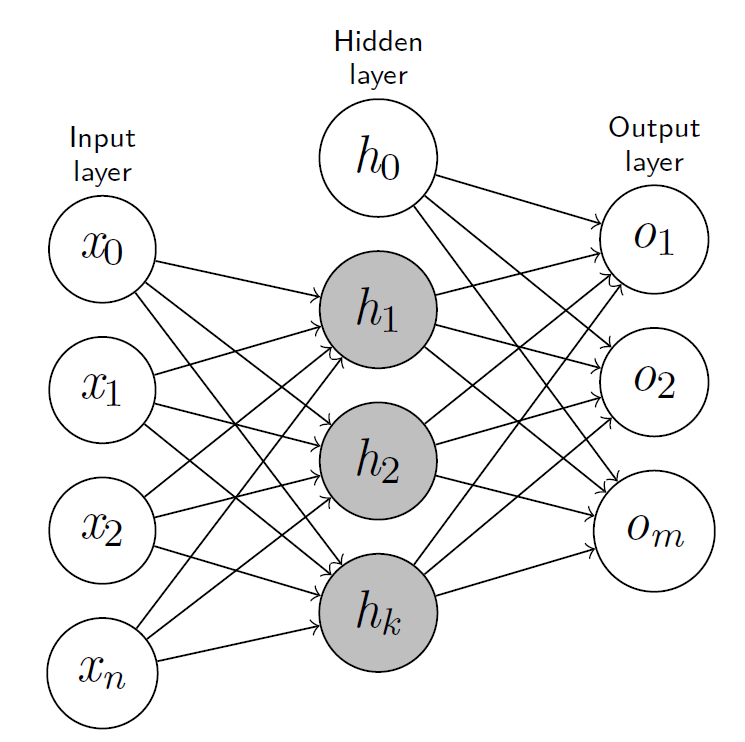
\includegraphics[width=0.18\columnwidth]{../imgs/nn_01.png}
    \end{figure}

    $o = f(W_1 \cdot f(W_0 \cdot x + b_0) + b_1)$, where $f$ is the activation function, applied element-wise.\\

    \textbf{Note:} The last activation function should based on the desired outputs. (Eg: One-hot encoding, regression)
        
\end{frame}

%-------------------------------------------------------------------------------
\section{Activation Functions}
\begin{frame}
    \frametitle{Activation Functions}
    
    The activation function must be \textbf{non-linear}.\break

    For a given non-input node $h$:
    \begin{itemize}
        \item Suppose there are $n$ nodes connect to $h$.
        \item Let $x$ be the column vector input to the node, that $x = (x_0, x_1, \ldots, x_n)^T$, where $x_0=1$.
        \item Let $w$ be the weights on the incident edges, that $w = (w_0, w_1, \ldots, w_n)^T$, where $w_0=b$ is the bias.
    \end{itemize}

    The output from this node is given by:

    \[
        f(w^T x) = f(\sum_{i=0}^n w_i x_i) = f(\sum_{i=1}^n w_i x_i + b)
    \]

    Where $f$ is the activation function for this node.\break

    If the activation function is linear, we can merge multiple hidden layers into one layer.
    The structure is equivalent to linear regression.
\end{frame}

%-------------------------------------------------------------------------------
\begin{frame}
    \frametitle{Sigmoid Function}

    \begin{figure}
        \centering
        \resizebox{0.35\columnwidth}{!}{
            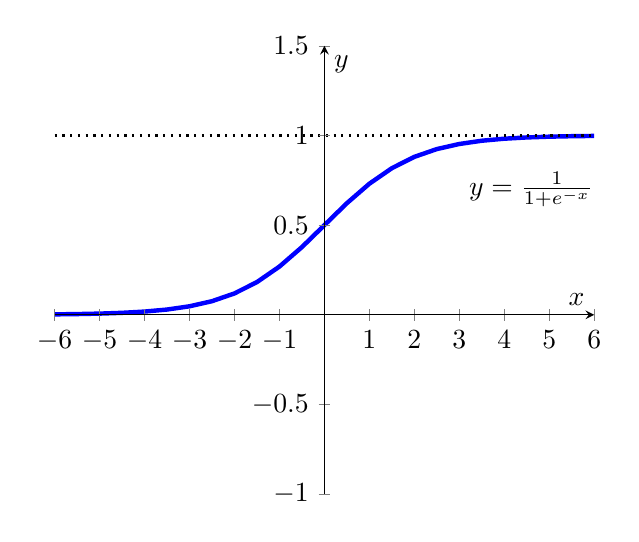
\begin{tikzpicture}
                \begin{axis}[
                        xmin=-6, xmax=6,
                        ymin=-1, ymax=1.5,
                        axis lines=center,
                        axis on top=true,
                        domain=-6:6,
                        ylabel=$y$,
                        xlabel=$x$,
                        xtick distance=1,
                        ytick distance=0.5
                    ]
                
                    \addplot [mark=none,draw=blue,ultra thick] {1/(1+exp(-\x))};
                    \node [right, black] at (axis cs: 3,0.7) {$y = \frac{1}{1+e^{-x}}$};
                    
                    \draw [black, dotted, thick] (axis cs:-6,1)-- (axis cs:6,1);
                    % \draw [black, dotted, thick] (axis cs:-6,0)-- (axis cs:6,0);
                \end{axis}
            \end{tikzpicture}    
        }
    \end{figure}

    \[
        f(x) = \text{Sigmoid}(x) = \sigma(x) = \frac{1}{1 + e^{-x}}
    \]

    Where $f(x) \in (0, 1)$, and the derivative is $f'(x) = f(x)(1- f(x))$.\\
    Rarely used in hidden layers for state-of-the-art models.\\
    Often used in the last hidden layer to produce logistic outputs.
\end{frame}

%-------------------------------------------------------------------------------
\begin{frame}
    \frametitle{Hyperbolic Tangent (tanh) Function}

    \begin{figure}
        \centering
        \resizebox{0.35\columnwidth}{!}{
            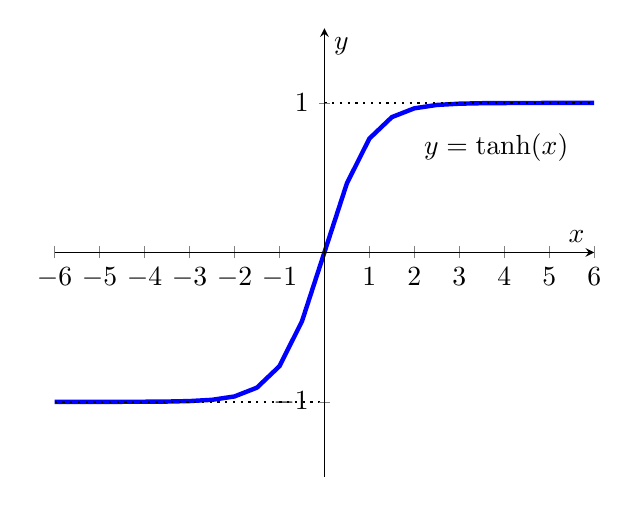
\begin{tikzpicture}
                \begin{axis}[
                        xmin=-6, xmax=6,
                        ymin=-1.5, ymax=1.5,
                        axis lines=center,
                        axis on top=true,
                        domain=-6:6,
                        ylabel=$y$,
                        xlabel=$x$,
                        xtick distance=1,
                        ytick distance=1
                    ]
                
                    \addplot [mark=none,draw=blue,ultra thick] {tanh(\x)};
                    \node [right, black] at (axis cs: 2,0.7) {$y = \tanh (x)$};
                    
                    \draw [black, dotted, thick] (axis cs:-6,-1)-- (axis cs:0,-1);
                    \draw [black, dotted, thick] (axis cs:0,1)-- (axis cs:6,1);
                \end{axis}
            \end{tikzpicture}    
        }
    \end{figure}

    \[
        f(x) = \tanh(x) = \frac{\sinh(x)}{\cosh(x)} = \frac{e^x - e^{-x}}{e^x + e^{-x}}
    \]
    
    Where $f(x) \in (-1, 1)$, and the derivative is $f'(x) = 1 - f(x)^2$\\
    Similar to Sigmoid function, but faster to converge.
\end{frame}

%-------------------------------------------------------------------------------
\begin{frame}
    \frametitle{Rectified Linear Unit (ReLU) Function}
    \small
    \begin{figure}
        \centering
        \resizebox{0.275\columnwidth}{!}{
            \begin{tikzpicture}
                \begin{axis}[
                        xmin=-2, xmax=2,
                        ymin=-1, ymax=2,
                        axis lines=center,
                        axis on top=true,
                        domain=-2:2,
                        ylabel=$y$,
                        xlabel=$x$,
                        xtick distance=1,
                        ytick distance=1
                    ]
                
                    \addplot+[mark=none,draw=blue,ultra thick,domain=-2:0] {0};
                    \addplot+[mark=none,draw=blue,ultra thick,domain=0:2] {\x};
                    
                \end{axis}
            \end{tikzpicture}    
        }
    \end{figure}

    \[
        f(x) = \text{ReLU}(x) = (x)^+ = \max(0, x)
    \]

    Where $f(x) \in [ 0, +\infty )$. The derivative is equal to:
    \[
        f'(x) = \begin{cases}
            0,& \text{if } x < 0 \\
            1,& \text{if } x > 0
        \end{cases}
    \]
    Where $x = 0$ is not differentiable.\\
    ReLU is the most common activation function for hidden layers in recent deep learning.

\end{frame}

%-------------------------------------------------------------------------------
\begin{frame}
    \frametitle{Leaky ReLU}
    \small
    \begin{figure}
        \centering
        \resizebox{0.275\columnwidth}{!}{
            \begin{tikzpicture}
                \begin{axis}[
                        xmin=-2, xmax=2,
                        ymin=-1, ymax=2,
                        axis lines=center,
                        axis on top=true,
                        domain=-2:2,
                        ylabel=$y$,
                        xlabel=$x$,
                        xtick distance=1,
                        ytick distance=1
                    ]

                    \node [right, black] at (axis cs: -2,-0.5) {$\epsilon = 0.1$};
                
                    \addplot+[mark=none,draw=blue,ultra thick,domain=-2:0] {0.1*\x};
                    \addplot+[mark=none,draw=blue,ultra thick,domain=0:2] {\x};
                    
                \end{axis}
            \end{tikzpicture}    
        }
    \end{figure}
    Let $\epsilon$ be the negative slope:
    \[
        f(x) = \text{LeakyReLU}(x) = \max(0, x) + \epsilon \times \min(0, x) = \begin{cases}
            x,& \text{if } x \geq 0\\
            \epsilon \times x,& \text{otherwise}
        \end{cases}
    \]
    Where $f(x) \in \rm$, and $\epsilon \in [0, 1)$ The derivative is equal to ($x = 0$ is not differentiable):
    \[
        f'(x) = \begin{cases}
            \epsilon,& \text{if } x < 0 \\
            1,& \text{if } x > 0
        \end{cases}
    \]
    Similar to ReLU, but overcomes the ``dead neuron'' problem.
\end{frame}

%-------------------------------------------------------------------------------
\section{Loss Functions}
\begin{frame}
    \frametitle{Loss Functions / Cost Function}
        
\end{frame}

%-------------------------------------------------------------------------------
\section{Optimization}
\begin{frame}
    \frametitle{Optimization}
        
\end{frame}

%-------------------------------------------------------------------------------
\section{Regularization}
\begin{frame}
    \frametitle{Dropout Layers}
        
\end{frame}

%-------------------------------------------------------------------------------
\section{Different Types of Layers}
\begin{frame}
    \frametitle{Convolution Layers}
        
\end{frame}

%-------------------------------------------------------------------------------
\begin{frame}
    \frametitle{Pooling Layers}
        
\end{frame}

%-------------------------------------------------------------------------------
\begin{frame}
    \frametitle{Recurrent Layers}
        
\end{frame}

%-------------------------------------------------------------------------------
\begin{frame}
    \frametitle{Transformer Layers}
        
\end{frame}

%-------------------------------------------------------------------------------
\section{Tutorial Questions}
\begin{frame}
    \frametitle{Tutorial Questions}
        
\end{frame}

\end{document}
